%\chapter{開発プロセス}
\section{第3サイクル}
第3サイクルは後期が始まった9月25日から10月21日に行われた外部講師によるリモートレビューまでとした。本サイクルでは、第2サイクルで見つかった大きな課題の一つである写真を撮る行為にもっとワクワクするような付加価値を加えなければならないこと、そして観光情報をより魅力的に紹介することを課題として活動を進めた。
\par まず我々は、後期が始まって最初のプロジェクト学習で前期を振り返り、もう一度課題を見直した。そして観光情報の表示の仕方について話し合った時、「札幌でしかできない50のこと」と言うネットの記事があるということを知り、それを参考にして木古内で「できること」に着目した情報の紹介する形式にすることを決定した。また、それと同時に「アプリからトランプを作れたら面白いのでは」と言う意見が出たため、そのアイディアを膨らませて、撮った写真を利用してカルタという「もの」にする機能を作ることも決定した。この時、リモートレビューまでには出来る範囲までは実装を行おうということで、木古内で「できること」に着目した情報紹介の機能から実装を進めた。具体的に修正した内容を表5.2に、実装はこの時マージが完了していなかったので、完成した画面イメージと印刷して完成したカルタのサンプルを図5.5、5.6に示す。それと同時に、アプリ内で紹介する観光スポットの写真を集めるために10月15日にメンバーでもう一度木古内へ行き、写真の素材を集めた。パンフレットやWebで掲載されていないような自分たちが見つけた魅力のあるスポットの写真も撮影できた。さらに、本サイクルでまだ決めていなかったアプリのタイトルをメンバー間で話し合った結果、「キーコ紀行」と呼ぶことを正式に決定した。
\par 本サイクルではより魅力的に観光情報が表示でき、写真を撮る動機づけとなるアイデアを練れた。しかし、カルタは50枚を超える紙を印刷するのは手間がかかるという課題が残った。また、技術面としてはメンバーで割り振った機能と機能をマージして一つのアプリにすることが課題となった。アプリを当時の直近のイベントであったアカデミックリンクに開発を間に合わせるようにスケジュールを立てることを決定した。

\begin{table}[htb]
\centering
\addtocounter{table}{+0}
\caption{第2サイクルから第3サイクルへの変化}
  \begin{tabular}{|l|l|} \hline
    改正前&改正後  \\ \hline 
    カテゴリごとに写真の一覧を表示 & \parbox{20zw}{写真と同時に紹介文を加えることで木古内で「できること」に着目した情報を表示} \\  \hline
    詳細情報を表示してからマップに遷移 &\parbox{20zw}{マップ画面と同時に詳細情報や写真を表示}\\ \hline
    「フォトストーリ―」という機能でアプリ内で写真を振り返る & \parbox{20zw}{カルタという「もの」にして思い出を残す}\\ \hline
  \end{tabular} 
\end{table}

\begin{figure}[htbp]
  \begin{center}
    \begin{tabular}{c}

      % 1
      \begin{minipage}{0.33\hsize}
        \begin{center}
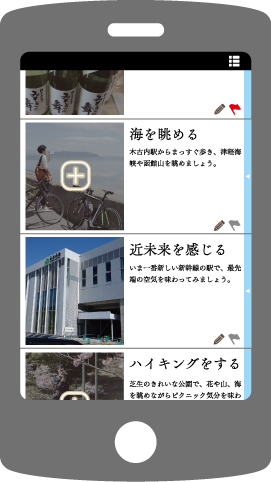
\includegraphics[width=4cm, bb=0 0 320 552]{appIdea1.png}
          \hspace{1cm} (a)観光スポットの紹介
        \end{center}
      \end{minipage}

      % 2
      \begin{minipage}{0.33\hsize}
        \begin{center}
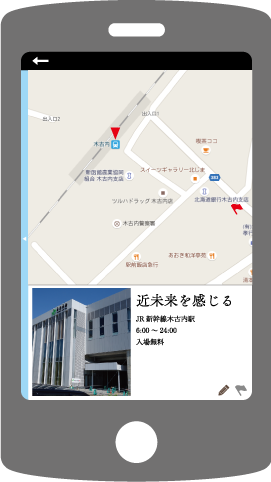
\includegraphics[width=4cm, bb=0 0 321 547]{appIdea2.png}
          \hspace{1cm} (b)詳細情報の表示
        \end{center}
      \end{minipage}

      % 3
      \begin{minipage}{0.33\hsize}
        \begin{center}
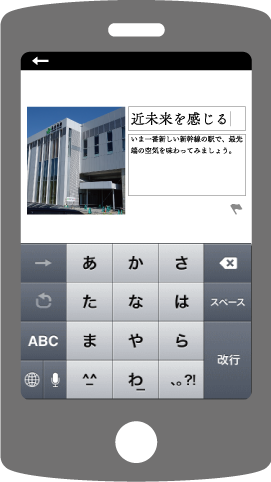
\includegraphics[width=4cm, bb=0 0 320 548]{appIdea3.png}
          \hspace{1cm} (c)紹介文の編集
        \end{center}
      \end{minipage}

    \end{tabular}
    \caption{第3サイクルの完成画面イメージ}
    \label{fig:lena}
  \end{center}
\end{figure}

\begin{description}
\item[カルタにする意義]\mbox{}
 \begin{itemize}
 \item iPhoneという小さい画面の中で振り返る必要が無い。
 \item 写真だけでなく、言葉と一セットになる形式を持っているため、より強く思い出を振り返ることが出来る。
 \item 実際に「もの」という形にすることで長く保管されやすい。
 \item 遊びながら思い出を振り返られる。
 \end{itemize}
\item[本サイクルの提案に対するレビュー内容]\mbox{}
 \begin{itemize}
 \item 「できること」に着目したことによって「どこに行こう?」から「ここに行きたい!」に近づいた。
 \item 実際に印刷する段階まで行ってほしい。
 \item 類似サービス(例えばFUJIFILMのフォトブック)の観光版のフォトブックとして作ってみるのは良い。
 \item ニーズはあると思う。
 \item ただ図5.6のようなカルタとは違う別の何かにした方が良い。手間がかかるから。
 \item 写真のプロトタイプを作って木古内の関係者に見せることで提案するのも良い。まずは見てもらうことが重要。
 \end{itemize}
\end{description}

\begin{figure}[htbp]
  \begin{center}
    \begin{tabular}{c}

      % 1
      \begin{minipage}{0.33\hsize}
        \begin{center}
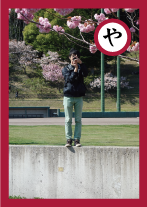
\includegraphics[width=4cm, bb=0 0 320 552]{karuta1.png}
        \end{center}
      \end{minipage}

      % 2
      \begin{minipage}{0.33\hsize}
        \begin{center}
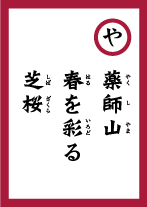
\includegraphics[width=4cm, bb=0 0 321 547]{karuta3.png}
        \end{center}
      \end{minipage}

      % 3
      \begin{minipage}{0.33\hsize}
        \begin{center}
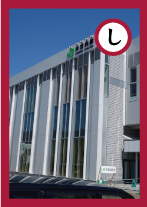
\includegraphics[width=4cm, bb=0 0 320 548]{karuta2.png}
        \end{center}
      \end{minipage}

    \end{tabular}
  \end{center}
\addtocounter{figure}{+0}
 \caption{カルタの完成サンプル}
\end{figure}

\bunseki{山川拓也}